\section{Rudin Chapter 15}

See also Stein II, Chapter 5.

\subsection{Jensen's formula}

\begin{lemma}
\[
\frac{1}{2\pi}\int_{0}^{2\pi} \log \lvert 1-e^{ i\theta } \rvert  \, \mathrm{d}\theta=0 
\]
\end{lemma}
\begin{proof}
\begin{figure}[H]
\centering
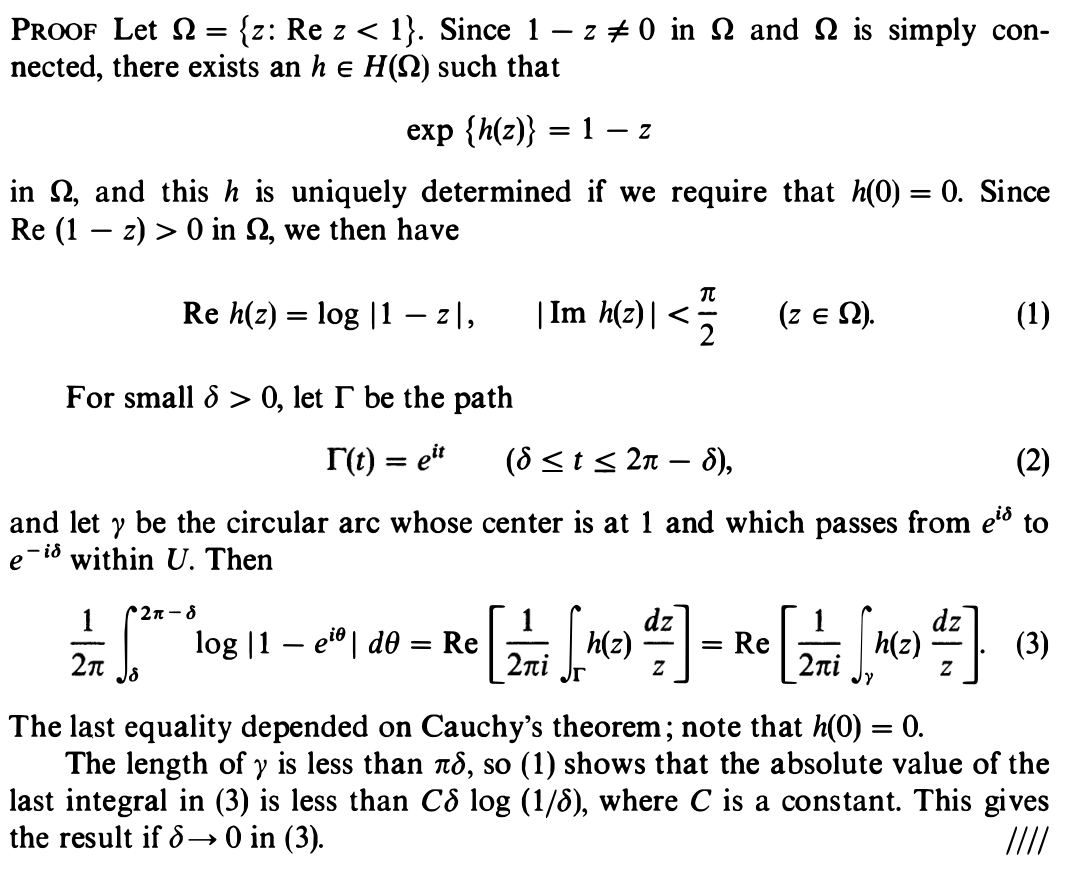
\includegraphics[width=\textwidth]{1-rudin-zeros-of-holomorphic-functions-2025052223.png}
% \caption{}
\label{}
\end{figure}
\end{proof}

\begin{figure}[H]
\centering
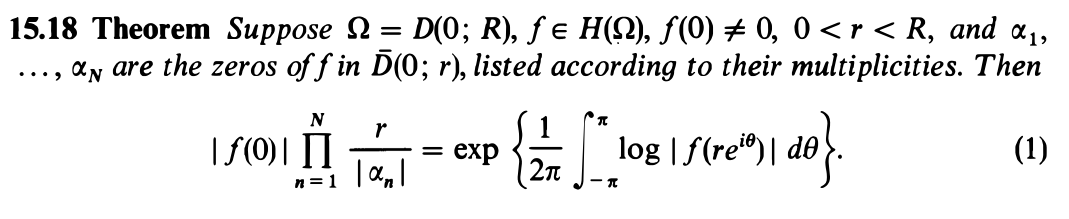
\includegraphics[width=\textwidth]{2-rudin-zeros-of-holomorphic-functions-2025052223.png}
% \caption{}
\label{}
\end{figure}

\begin{note}
This is known as Jensen's formula. The hypothesis $f(0) \neq 0$ causes no harm in applications, for if $f$ has a zero of order $k$ at $0$, the formula can be applied to $f(z)/z^k$.
\end{note}
\begin{proof}
\begin{figure}[H]
\centering
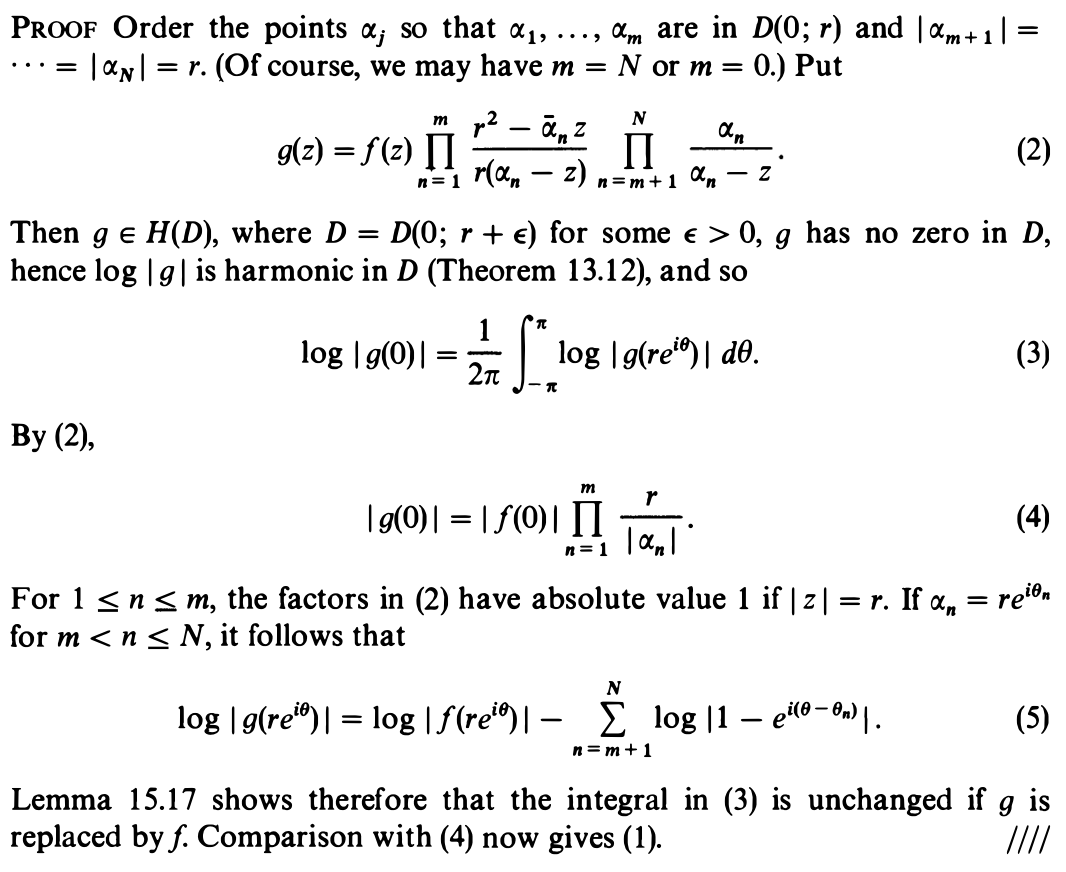
\includegraphics[width=\textwidth]{4-rudin-zeros-of-holomorphic-functions-2025052223.png}
% \caption{}
\label{}
\end{figure}
\end{proof}

\subsubsection{Applications of Jensen's formula: zeros of entire function}

\begin{figure}[H]
\centering
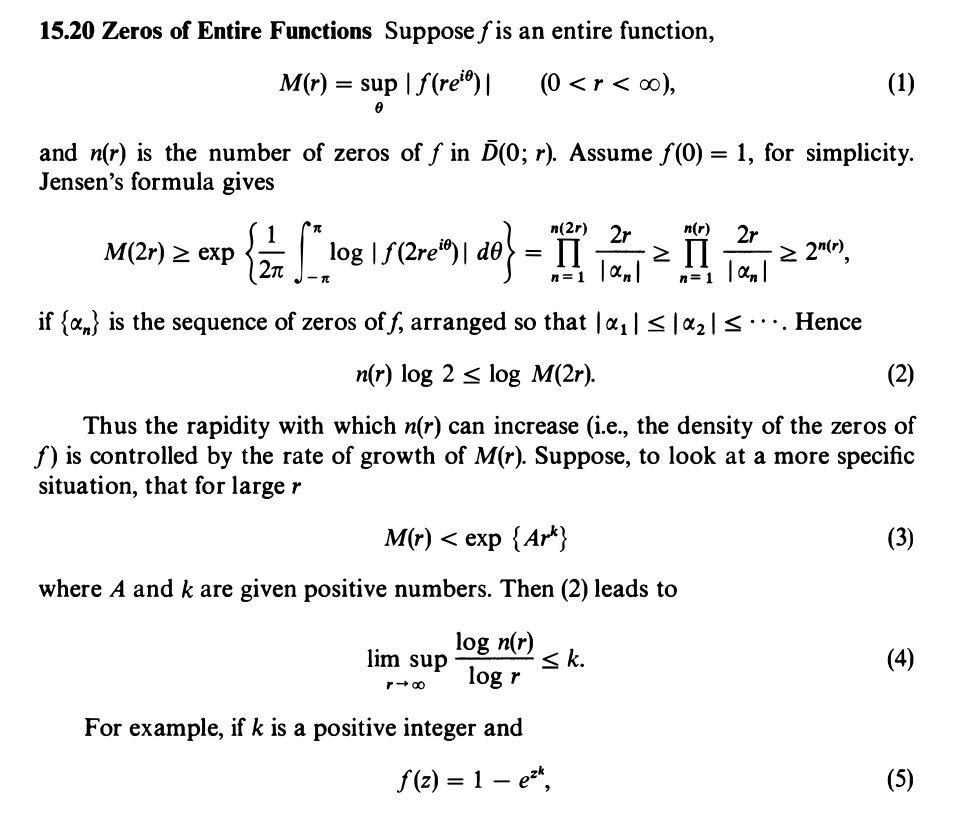
\includegraphics[width=\textwidth]{rudin-zeros-of-holomorphic-functions-2025061922.png}
% \caption{}
\label{}
\end{figure}
\begin{figure}[H]
\centering
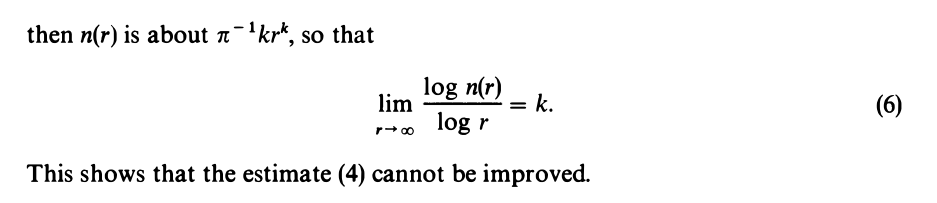
\includegraphics[width=\textwidth]{1-rudin-zeros-of-holomorphic-functions-2025061922.png}
% \caption{}
\label{}
\end{figure}
